\documentclass{article}
\usepackage[margin=1in]{geometry}
\usepackage[utf8]{inputenc}
\usepackage{graphicx} 
\usepackage{fancyhdr}
\usepackage{enumitem}
\usepackage{lipsum}
\usepackage[bahasa]{babel}
\usepackage{subcaption}
\usepackage{float}
\usepackage{indentfirst}

\title{Laporan Workshop Telematika \\ Dasar Desain 3D Model Fusion 360} % Ganti sesuai modul praktikum yang diikuti
\author{Azaria Putri Fawnia \\ 5024221038} % Ganti dengan NRP dan Nama Kalian

\date{}


\fancypagestyle{firstpageheader}{
  \fancyhf{} 
  \fancyhead[L]{
\includegraphics[height=1.5cm]{img/modul_1/logodepart.png}} 
  \fancyhead[R]{Institut Teknologi Sepuluh Nopember \\ Departemen Teknik Komputer \\ Laboratorium Robotika dan Sistem Cerdas} 
  \renewcommand{\headrulewidth}{0pt} 
  \fancyfoot[C]{%
    
\includegraphics[width=\textwidth]{img/modul_1/footer.png}
  }
  \renewcommand{\footrulewidth}{0pt} % No line in the footer
}


\fancyhf{} 
\fancyfoot[C]{%
  
\includegraphics[width=\textwidth]{img/modul_1/footer.png}
}
\renewcommand{\headrulewidth}{0pt} 
\renewcommand{\footrulewidth}{0pt} 

\pagestyle{fancy}
\begin{document}
\selectlanguage{bahasa}
\maketitle
\thispagestyle{firstpageheader}
% Bagian Tugas Pendahuluan
\section*{Tugas Pendahuluan}
\begin{enumerate}
  \item Buat satu desain kubus pada fusion 360 seperti pada gambar di modul 3 \\
  \begin{figure}[H]
    \centering
    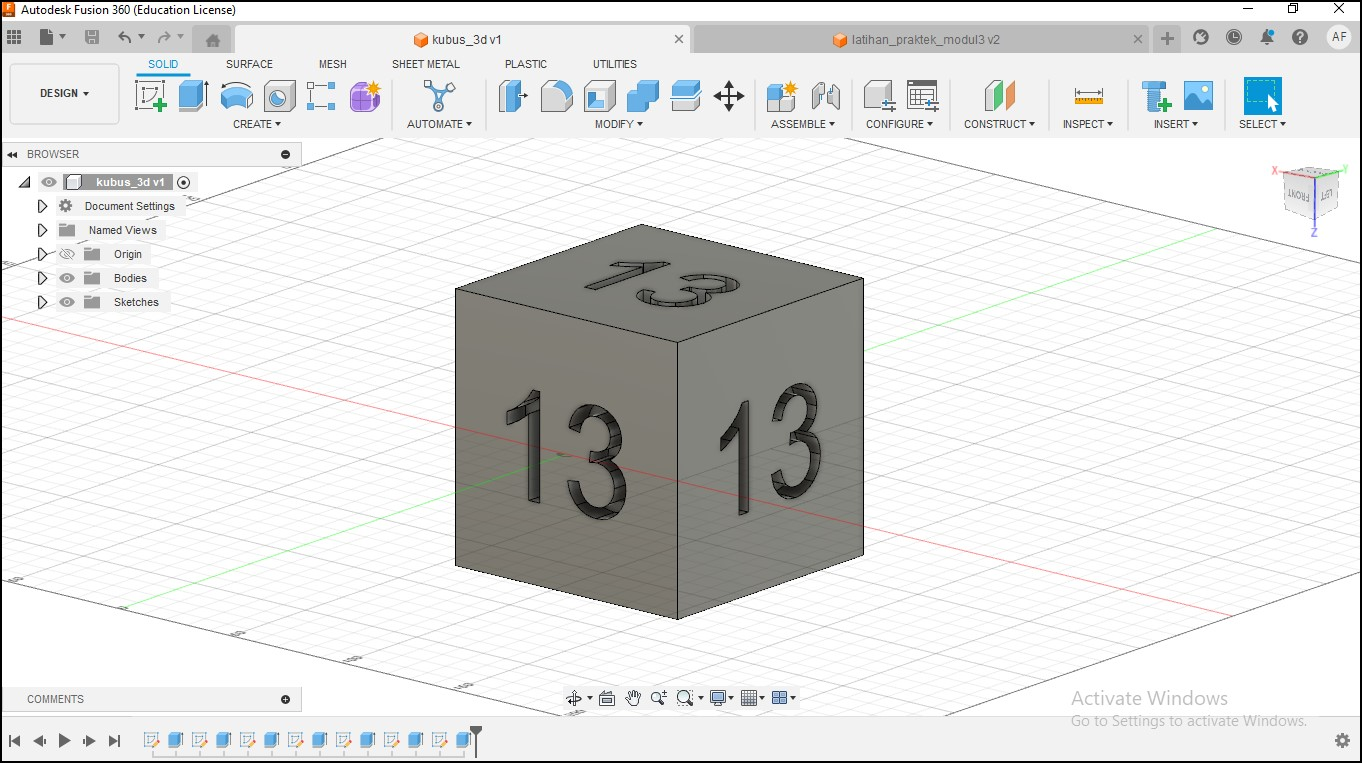
\includegraphics[width=0.7\linewidth]{img/modul_3/tupen3_kubus.jpg}
    \caption{Bukti hasil desain kubus pada fusion 360} 
  \end{figure}
  \item Install Ultimaker CURA \\
  \begin{figure}[H]
    % Kalau mau menambah gambar lagi tinggal nambahin begin{subfigure} -> end{subfigure}
    \centering
    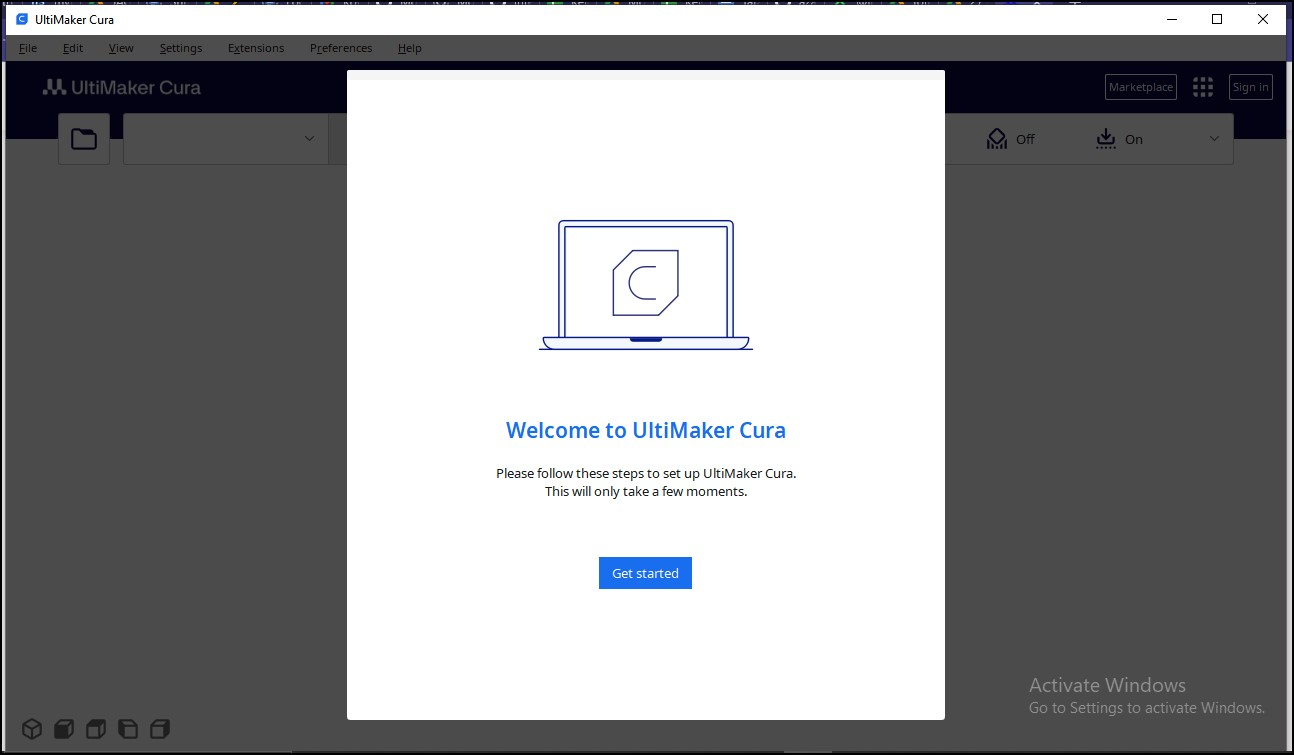
\includegraphics[width=0.6\linewidth]{img/modul_3/tupen3_install_cura.jpg}
    \caption{Bukti desain PCB\label{fig:inisub1}}
  \end{figure}
  \item Pahami tentang penggunaan Ultimaker CURA untuk print 3d \\
\end{enumerate}
  


% Bagian Analisis Hasil Percobaan
\section*{Analisis Hasil Percobaan}
\indent
Pada Percobaan modul 1 WORKSHOP Telematika, workshop dimulai dengan membuat rangkaian schematics minimum system ESP8266 yang dilakukan dengan mengikuti langkah-langkah yang sudah dicantumkan di modul. Proses membuat rangkaian schematic ini menggunakan komponen-komponen yang terdapat pada library yang sudah disediakan oleh aslab. Setelah proses membuar rangkaian schematic selesai, kemudian dibuat PCB dari schematic tersebut. Setelah proses wiring koneksi selesai kita mendapatkan hasil PCB yang siap di gunakan.

% \begin{table}[h]
%     \centering
%     \caption{Caption tabelnya}
%     \label{tab:labelini}
%     \begin{tabular}{|c|c|c|c|}
%     \hline
%     Kolom 1 & Kolom 2 & Kolom 3 & Kolom 4 \\
%     \hline
%     Data 1 & Data 2 & Data 3 & coba nambah kolom \\
%     Data 4 & Data 5 & Data 6 & coba nambah kolom juga \\ 
%     \hline
%     \end{tabular}
% \end{table}
% Bagian Lampiran
\section*{Lampiran} % Jika ada lampiran

% ini buat percobaan 1

\begin{figure}[H]
  \centering
  % Kalau mau menambah gambar lagi tinggal nambahin begin{subfigure} -> end{subfigure}
  \begin{subfigure}[c]{0.4\linewidth}
    \centering
    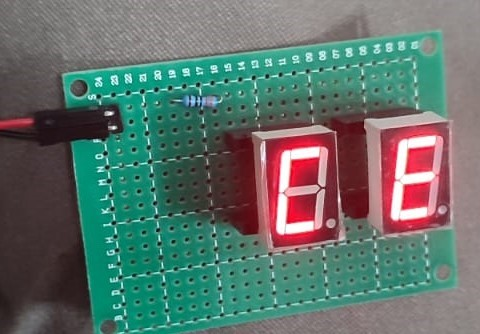
\includegraphics[width=\linewidth]{img/modul_2/percobaan1_hasil.jpg}
    \caption{Hasil 7 segment saat dinyalakan\label{fig:inisub1}}
  \end{subfigure}
  \hspace{1cm}
  \begin{subfigure}[c]{0.4\linewidth}
    \centering
    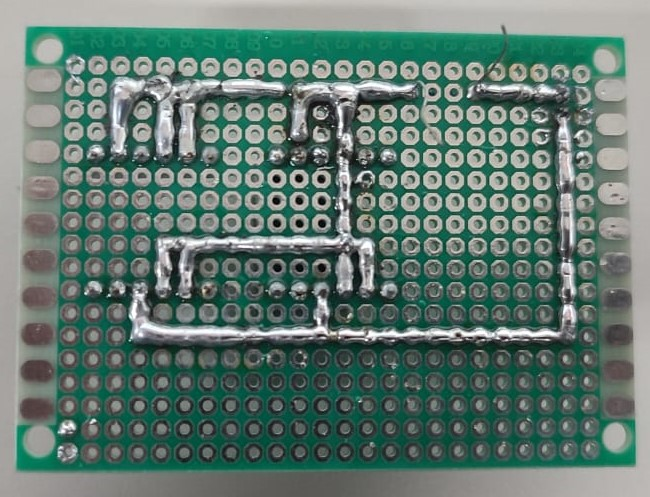
\includegraphics[width=\linewidth]{img/modul_2/percobaan1_hasil_solder.jpg}
    \caption{Hasil soldering PCB (tampak belakang) \label{fig:inisub2}}
  \end{subfigure}
  \caption{Hasil percobaan 1 \label{fig:keduagambar}}
\end{figure}

\begin{figure}[H]
  \centering
  % Kalau mau menambah gambar lagi tinggal nambahin begin{subfigure} -> end{subfigure}
  \begin{subfigure}[c]{0.4\linewidth}
    \centering
    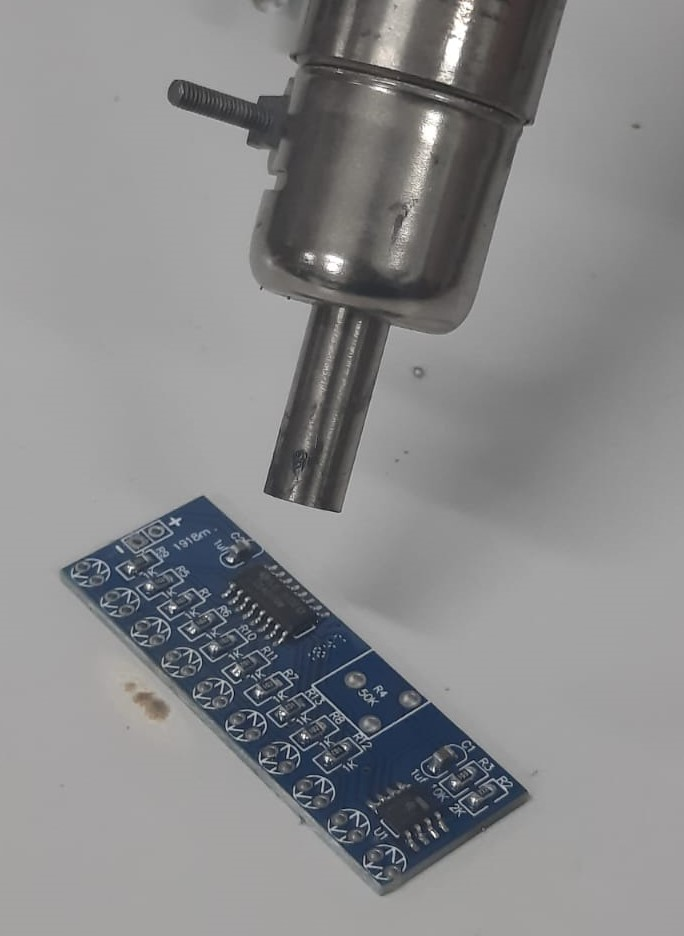
\includegraphics[width=\linewidth]{img/modul_2/percobaan2_soldering_uap.jpg}
    \caption{Proses soldering PCB menggunakan solder uap \label{fig:inisub1}}
  \end{subfigure}
  \hspace{1cm}
  \begin{subfigure}[c]{0.4\linewidth}
    \centering
    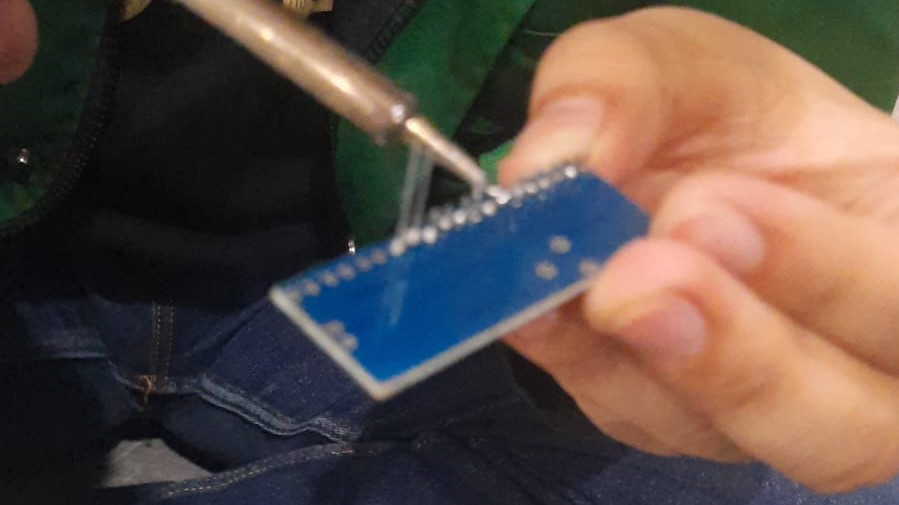
\includegraphics[width=\linewidth]{img/modul_2/percobaan2_soldering_biasa.jpg}
    \caption{Proses soldering PCB menggunakan solder biasa \label{fig:inisub2}}
  \end{subfigure}
  \caption{Proses soldering pada komponen percobaan 2 \label{fig:keduagambar}}
\end{figure}

\begin{figure}[H]
  \centering
  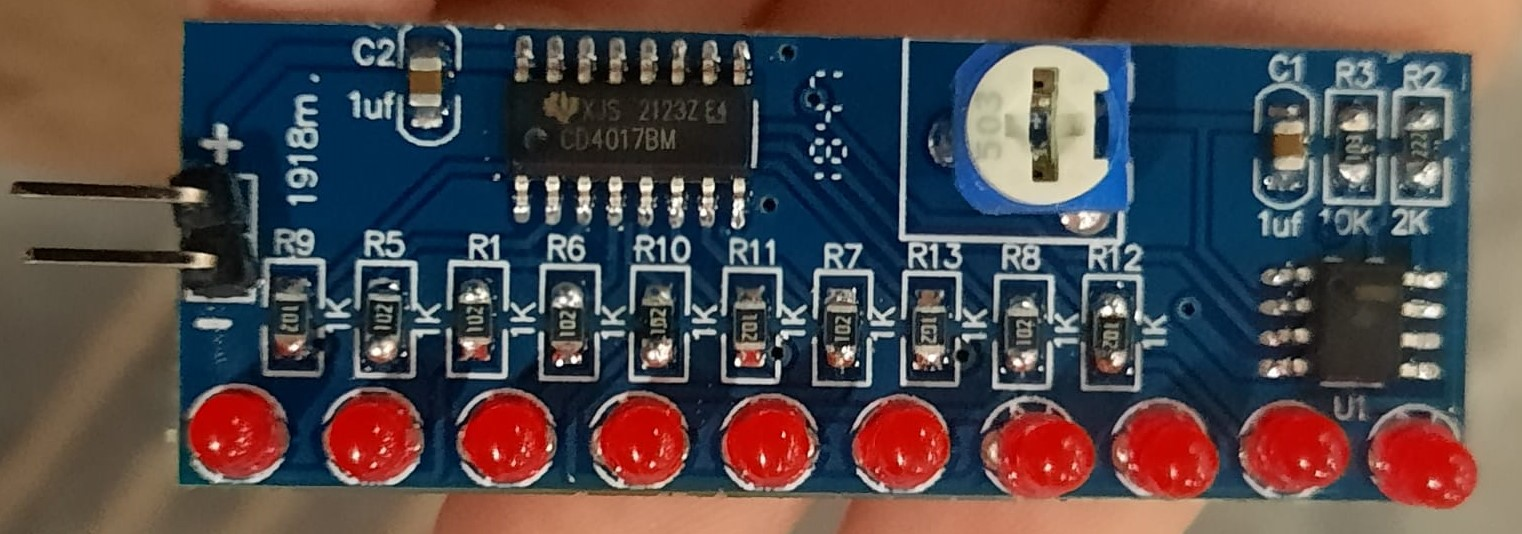
\includegraphics[width=0.7\linewidth]{img/modul_2/percobaan2_hasil.jpg}
  \caption{Hasil percobaan 2 \label{fig:inisub1}}
\end{figure}
\end{document}